\documentclass{article}
\usepackage{graphicx}
\usepackage{amsmath}
\usepackage[mathletters]{ucs}
\usepackage[utf8x]{inputenc}
\usepackage{listings}
\lstnewenvironment{code}{\lstset{language=Haskell,basicstyle=\small\ttfamily}}{}

\setlength{\parindent}{0pt}
\setlength{\parskip}{6pt plus 2pt minus 1pt}

\usepackage{pgf, tikz}
\usetikzlibrary{shapes}
\usetikzlibrary{shapes.multipart}
\usetikzlibrary{arrows}

\lstdefinelanguage{FSharp}
      {morekeywords={let, new, match, inherit, abstract, with, rec,
          open, module, namespace, type, of, member, and, for, in, do,
          begin, end, fun, function, try, mutable, if, then, else,
          class, interface, end},
    keywordstyle=\color{blue},
    basicstyle = \small,
    sensitive=false,
    morecomment=[l][\color{green!50!black!80}]{///},
    morecomment=[l][\color{green!50!black!80}]{//},
    morecomment=[s][\color{green!50!black!80}]{{(*}{*)}},
    morestring=[b]",
    stringstyle=\color{red},
    columns=fullflexible
    }


\lstdefinelanguage{Smalltalk}{
  basicstyle=\ttfamily,
  keywordstyle=\bfseries,
  morekeywords={self,super,true,false,nil,thisContext}, % This is overkill
  morestring=[d]',
  morecomment=[s]{"}{"},
  alsoletter={\#:},
  escapechar={!},
}[keywords,comments,strings]


\newcommand{\Blue}[1]{\color{blue}#1\color{black}\xspace}


\usepackage{array}
% This is needed because raggedright in table elements redefines \\:
\newcommand{\PreserveBackslash}[1]{\let\temp=\\#1\let\\=\temp}
\let\PBS=\PreserveBackslash

%%%%%%%%%%%%%% 
%\newcommand{\solution}[1] {}
\newcommand{\solution}[1] {\textbf{Solutions:}\\ #1}

%\newcommand{\comment}[1]{}
\newcommand{\comment}[1]{\marginpar{#1}}


\begin{document}
\newcommand{\examtime}{14:00, Thursday August 18th, 2010}
\newcommand{\points}[1]{\marginpar{\bf #1 points}}
\noindent
\begin{tabular}{lr}
CHALMERS TEKNISKA H\"OGSKOLA &\examtime{}.\\
Dept. of Computer Science and Engineering & Programming Paradigms\\
John Hughes                  & DAT120 / DIT330(GU) \\
\end{tabular}

\vspace{2.5cm} \noindent
\begin{center} {\LARGE
Exam in Programming Paradigms}
\end{center}

\vspace{1.5cm}

\noindent
\examtime{}.\\
\begin{tabular}{lllc}
\textbf{Lecturer:} &  John Hughes  & tel 070 756 3760 & (Examiner)\\
\textbf{Lecturer:} & Richard Bubel & tel 073 965 7355 & \\ 
\end{tabular}
\vspace{1cm}

\noindent
Permitted aids:\\
English-Swedish or English-other language dictionary.

There are 5 questions on {\Huge to be filled in} numbered pages. 

Five of the six questions are ordinary questions: One on functional
programming (12 points), one on concurrency oriented programming (12
points), one on basic imperative and object-oriented concepts (12
points), one on object-oriented programming (12 points) and one on
logic programming (12 points).

The total sum is 60 points.


\textbf{Chalmers:}
24 points is required to pass (grade 3), 36 points is required for
grade 4, and 48 points is required for grade 5. 

\textbf{GU:}
24 points is required to pass (grade G) and 48 points is required for
grade VG.


\newpage 
\hfill\\
\newpage


\newpage

\section{Basic Imperative and Object-Oriented Concepts [12 points]}
\lstset{language=Java, columns=flexible}

\begin{enumerate}
\item Describe the computation workflow of the \emph{von Neumann
    computing model}.\points{2}
\item Let \lstinline!A! be a class with an integer typed attribute
  \lstinline!a!.
\begin{lstlisting}[language=Java, columns=flexible]
class A {  int a;  }
\end{lstlisting}

and the following program fragment
\begin{lstlisting}[language=Java, columns=flexible] 
A x; A y;
...
// x and y point to different objects
x.a = 1;
y.a = 5;

x = y;

x.a = x.a + y.a;   
y.a = x.a - y.a;
x.a = x.a - y.a; (*)
\end{lstlisting}
where the program variables \lstinline!x! and \lstinline!y! refer
initially to different objects.

Give the values of \lstinline!x.a! and \lstinline!y.a! after execution
of line \lstinline!(*)! if the assignment operator is realised using
\begin{enumerate}
  \item copy semantics 
  \item reference semantics 
\end{enumerate}
\points{2}
\item For what should the equality operator test to be compatible with
  an assignment operator implementing 
  \begin{enumerate}
  \item copy semantics?
  \item reference semantics?
 \end{enumerate}\points{1} 
\item Consider the following program:
\begin{lstlisting}[language=Java, columns=flexible] 
int g(int b, int c) {
  if (b < c) {
    return g(c,b); 
  }
  if ( c > 0 ) 
     return b + g(b, c - 1);
  }
  return 0; (*)
}
\end{lstlisting}

Consider the call 
\begin{center}
  \lstinline[language=Java, columns=flexible]{g(3, 5);} 
\end{center}
Give the number of activation records on the stack resulting from the
above call just before returning from (*), i.e., directly after
assigning the return value, but before popping the last activation
record from the stack. Give also the last two activation records on
top of the stack (the last allocated ones). State their order
explicitly and name all slots/components of the activation record and
their content explicitly. If a content is not yet defined use
'\texttt{?}' as value. \points{3}
\item Consider the following program
\begin{lstlisting}[language=Java, columns=flexible] 
void f(by-?? int a, by-?? int b, by-?? int c) {
  a = a + a;
  b = a + b + c;
  c = c + 15;
}

 ..
 int i, j;
 i = 1; 
 j = 5;
 f(i+1, i, j); //(*)
\end{lstlisting}

What are the values of the variables \lstinline!i! and \lstinline!j!
at (*) after the method \lstinline!f! returns if
\begin{enumerate}
  \item all parameters are passed \emph{by-copy}
  \item parameter \lstinline!a! is passed \emph{by-copy} and
    the parameters \lstinline!b! and \lstinline!c! \emph{by-reference}
  \item the parameters \lstinline!a! and \lstinline!b! are passed by
    copy and parameter \lstinline!c! \emph{by-value-result}. 
  \item parameter \lstinline!a! is passed \emph{by-name}, parameter
    \lstinline!b! is passed \emph{by-reference} and parameter
    \lstinline!c! is passed \emph{by-copy}.
\end{enumerate} \points{4}
\end{enumerate}

\solution{
\begin{enumerate}
\item (Each item below 0.5 points) The CPU 
  \begin{enumerate}
  \item  reads next instruction from memory (indexed by program counter PC)
    Memory
  \item fetches required data from memory
  \item operates on data
  \item writes result back to memory and updates PC
  \end{enumerate}
\item
  \begin{enumerate}   
  \item \lstinline!x.a!: 5 \quad  \lstinline!y.a!: 5
  \item \lstinline!x.a!: 0  \quad \lstinline!y.a!: 0
  \end{enumerate}
\item 4 activation records are on the stack; the last two ones
  $A_1$, $A_2$ where $A_2$ is the one on top of the stack are defined
  as follows: $A_1=(8,1,?,\text{ref to}~A_{0} , ?)$ (first two parameters,
  third local variable, fourth reference to first activation record,
  fifth return value), $A_2=(8,0, \text{ref to}~A_1, 0)$  
\item\hfill\\
  \begin{tabular}{lcc}
    & \lstinline!i! & \lstinline!j! \\ \hline
   (a) &  1 & 5 \\
   (b) & 10 & 20 \\
   (c) & 1 & 20 \\
   (d) & 14 & 5 \\
  \end{tabular}

  
\end{enumerate}
}

\newpage

\section{Object-Oriented Programming [12 points]}

\begin{enumerate}
\item Given two classes $A$ and $B$, where $B$ inherits from $A$. Both
  classes declare a field of the same name $f$.  Name and explain two
  possibilities to resolve such field name clashes.\points{2}
\item Explain the difference between replicated and shared
  inheritance. \points{2}
\item Given the following class
  hierarchy \\
\begin{center}

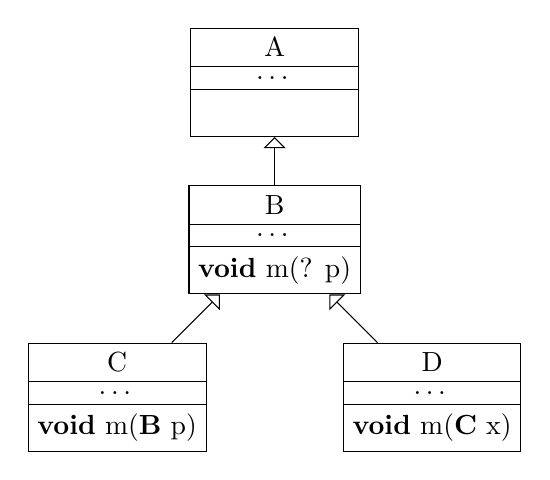
\begin{tikzpicture}
\node[draw, 
   rectangle split, 
   rectangle split parts=3, 
   minimum width=2cm] (A) at (5,4) 
  {A 
     \nodepart{second} \ldots 
     \nodepart{third} \phantom{\textbf{void} h(A x)}};
\node[draw, 
   rectangle split, 
   rectangle split parts=3, 
   minimum width=2cm] (B) at (5,2) 
  {B 
     \nodepart{second} \ldots 
     \nodepart{third} \textbf{void} m(? p)};
\node[draw, 
   rectangle split, 
   rectangle split parts=3, 
   minimum width=2cm] (C) at (3,0) 
  {C 
    \nodepart{second} \ldots 
    \nodepart{third} \textbf{void} m(\textbf{B} p)};   

\node[draw, 
   rectangle split, 
   rectangle split parts=3, 
   minimum width=2cm] (D) at (7,0) 
  {D 
     \nodepart{second} \ldots 
     \nodepart{third} \textbf{void} m(\textbf{C} x)};

\draw[open triangle 90-] (A) -- (B);
\draw[open triangle 90-] (B) -- (C);
\draw[open triangle 90-] (B) -- (D);
\end{tikzpicture}
\end{center}
defining all available classes. Note: Class \lstinline!A! does not
define any method.
Give for each of the following overriding semantics (for arguments):
\begin{enumerate}
  \item co-variance,
  \item contra-variance and
  \item invariance
\end{enumerate}
\emph{all} possible argument types for method
\lstinline!m! in class \lstinline!B! such that
\lstinline!m! is overridden by the method \lstinline!m! declared in
class \lstinline!C! and class \lstinline!D!. \emph{Hint:} There might
not be a solution for all semantics in that case write ``not possible''.  \comment{\textbf{3 points}}\newpage
\item Given the following class hierarchy:\\
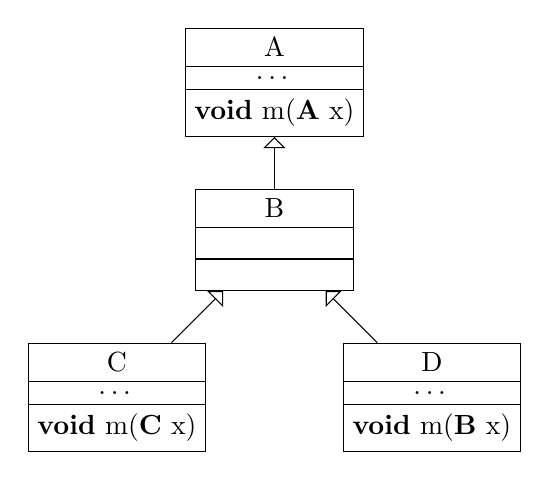
\begin{tikzpicture}
\node[draw, 
   rectangle split, 
   rectangle split parts=3, 
   minimum width=2cm] (A) at (5,6) 
  {   A 
     \nodepart{second} \ldots 
     \nodepart{third} \textbf{void} m(\textbf{A} x)};
\node[draw, 
   rectangle split, 
   rectangle split parts=3, 
   minimum width=2cm] (B) at (5, 4) 
  {   B 
  };

\node[draw, 
   rectangle split, 
   rectangle split parts=3, 
   minimum width=2cm] (C) at (3,2) 
  {C 
     \nodepart{second} \ldots 
     \nodepart{third} \textbf{void} m(\textbf{C} x)
  };
 \node[draw, 
    rectangle split, 
    rectangle split parts=3, 
    minimum width=2cm] (D) at (7,2) 
  {D
    \nodepart{second} \ldots 
    \nodepart{third} \textbf{void} m(\textbf{B} x)};   

\draw[open triangle 90-] (A) -- (B);
\draw[open triangle 90-] (B) -- (C);
\draw[open triangle 90-] (B) -- (D);
\end{tikzpicture}

The visibility of method \lstinline!m! is public. Overriding semantics
for methods is such that the method \lstinline!m!  of class
\lstinline!C! as well as the method \lstinline!m! of class
\lstinline!D! override the method \lstinline!m! defined in class
\lstinline!A!. Class \lstinline!B! does not (re-)implement method
\lstinline!m!.

In addition there is a method \lstinline!g! 
\begin{lstlisting}[language=Java, columns=flexible]
void g(A x, B y) {
   x.m(y);
}
\end{lstlisting}

Which of the three implementations of method \lstinline!m! is invoked by
\lstinline!g! if
\begin{enumerate}
\item the programming language uses \emph{single-dynamic dispatch} and
  the call statement is
 \begin{enumerate}
    \item \lstinline!g(new C(), new B());!
    \item \lstinline!g(new C(), new C());!
    \item \lstinline!g(new D(), new C());!
  \end{enumerate}
  \item the programming language uses \emph{multi-dynamic dispatch}
    and the call statement is
 \begin{enumerate}
    \item \lstinline!g(new C(), new D());!
    \item \lstinline!g(new C(), new C());!
    \item \lstinline!g(new D(), new C());!
    \end{enumerate}
\end{enumerate}\points{3}\newpage
\item Which of the following statements are true\\
    \begin{tabular}{|p{6cm}|c|c|}\hline
      & True & False \\ \hline
      a) F\# does not allow to declare new classes. It can only reuse
      existing ones to be able to interact with the \texttt{.net} environment. & & \\\hline
      b) In F\# mutable variables can be be assigned different values, whereas
      the values stored inside reference cells are immutable. & & \\\hline
      c) Current versions of F\# do not support concurrency. & & \\\hline
      d) In Smalltalk the only two types are integers and objects. & & \\\hline
   \end{tabular}\\
   For your answer draw that table but refer to the statements by a),
   b) etc. instead of writing them again. Wrong answers lead to a
   reduction of points, a negative result does not carry over to other
   sub-assignments. \points{2}
\end{enumerate}

\solution{
\begin{enumerate}
\item For example, by renaming (compiler error; programmer has to
  rename field explicitly) and/or shadowing (both field co-exist;
  complexer access rules)
\item \emph{Replicated Inheritance}: child object contains  multiple
  copies of fields/methods; 
  \emph{Shared (diamond)  Inheritance} child object contains only one
  superclass object.
\item 
    \begin{enumerate}
      \item A, B
      \item C
      \item not possible
    \end{enumerate}
\item 
    \begin{enumerate}
    \item 
    \begin{enumerate}
    \item method \lstinline!m! as defined in class \lstinline!A!
    \item method \lstinline!m! as defined in class \lstinline!A!
    \item method \lstinline!m! as defined in class \lstinline!D!
 \end{enumerate}
    \item 
    \begin{enumerate}
    \item method \lstinline!m! as defined in class \lstinline!A!
    \item method \lstinline!m! as defined in class \lstinline!C!
    \item method \lstinline!m! as defined in class \lstinline!A!
    \end{enumerate}
    \end{enumerate}
\item
      \begin{tabular}{|p{6cm}|c|c|}\hline
      & True & False \\ \hline
       a) F\# does not allow to declare new classes. It can only reuse
      existing ones to be able to interact with the \texttt{.net}
      environment. & & X \\\hline
      b) In F\# mutable variables can be be assigned different values, whereas
      the values stored inside reference cells are immutable. & & X \\\hline
      c) Current versions of F\# do not support concurrency. & & X \\\hline
      d) In Smalltalk the only two types are integers and objects. & &
      X \\\hline
   \end{tabular}\\

\end{enumerate}
}

\end{document}
